% Author: Izaak Neutelings (June 2022)
% Inspiration:
%   https://en.wikipedia.org/wiki/File:Electroweak.svg
%   https://commons.wikimedia.org/wiki/File:Standard_Model.svg
%   http://www.scientificlib.com/en/Physics/LX/WeakHypercharge.html % anti-fermions wrong ?
%   https://en.wikipedia.org/wiki/Mathematical_formulation_of_the_Standard_Model#Field_content_in_detail
%   https://en.wikipedia.org/wiki/C-symmetry#Charge_conjugation_in_the_chiral_basis
\documentclass[border=3pt,tikz]{standalone}
\usepackage{tikz}
\usepackage{amsmath} % for \text
\usepackage[outline]{contour} % glow around text
\usetikzlibrary{arrows.meta} % to control arrow size
\tikzset{>={Latex[length=4,width=4]}} % for LaTeX arrow head
\usetikzlibrary{calc}
\usepackage{xcolor} % for colored text
\contourlength{1.1pt}

\colorlet{myblue}{blue!70!black}
\colorlet{mydarkblue}{blue!40!black}
\colorlet{mypurple}{blue!60!red!80!black}
\colorlet{myred}{red!70!black}
\colorlet{myred2}{red!75!blue!80!black!90}
\colorlet{mydarkred}{red!50!black}
\colorlet{mygreen}{green!60!black}
\colorlet{mygreen2}{green!68!blue!70!black!90}
\colorlet{mydarkgreen}{green!30!black}
\colorlet{myorange}{orange!88!black}
\colorlet{myorange2}{orange!75!black}
\colorlet{myyellow}{yellow!80!orange!90!black}
\def\tick#1#2{\draw[thick] (#1) ++ (#2:1pt) --++ (#2-180:2pt)}
\renewcommand\bar{\overline}
\renewcommand\tilde{\widetilde}
\newcommand{\YW}{Y_\mathrm{W}}
\newcommand{\ff}[2]{#1_\text{#2}} % fermion field
\newcommand{\aff}[2]{\overline{#1}_\text{#2}} % anti-fermion field
\tikzstyle{guide}=[ultra thin,black!15,line cap=round]
\tikzstyle{myball}=[line width=0.05,ball color=#1]

% COMMON MACROS
\def\myball(#1)[#2]{
  \fill[ball color=#2] (#1) circle(\r);
  \fill[#2,opacity=0.4] (#1) circle(\r);
  \draw[draw=#2!20!black,line width=0.04] (#1) circle(\r)
}
\def\quark(#1)[#2]#3{
  \myball({#1)++(-30:0.8*\r})[red];
  \myball({#1)++(-150:0.8*\r})[green!88!black];
  \myball({#1)++(90:0.8*\r})[blue];
  %\draw[myball=red] (#1)++(-30:0.8*\r) circle(\r);
  %\draw[myball=green] (#1)++(-150:0.8*\r) circle(\r);
  %\draw[myball=blue] (#1)++(90:0.8*\r) circle(\r);
  \node[#2] at (#1) {\strut#3}
}
\def\barwidth{0.015} % doublet thickness
\def\doublet#1#2{\begin{pmatrix}#1\\#2\end{pmatrix}}
\def\drawdoublet[#1,#2](#3){% % rectangle with fading color
  \fill[#2,left color=#1,right color=#2]%
    (-1/2,#3)++(0,-\barwidth/2) rectangle++ (1,\barwidth)%
}
\def\drawtriplet[#1,#2](#3){% % rectangle with fading color
  \fill[#2,left color=#1,right color=#2]%
    (-1,#3)++(0,-\barwidth/2) rectangle++ (2,\barwidth)%
}

\begin{document}


% COMMON AXIS
\def\r{0.7pt} % point radius
\pgfmathsetmacro\qscale{1/sqrt(2)} % unit Q charge in (I3,YW/2)
\def\TQYaxis{
  
  % GUIDELINES
  \foreach \i [evaluate={\y=1.05*(1.2-abs(\i/2))}] in {1,2}{ % weak isospin T3
    \draw[guide] (-\i/2,-\y) -- (-\i/2,\y);
    \draw[guide] ( \i/2,-\y) -- ( \i/2,\y);
  }
  \foreach \i [evaluate={\x=0.9*(1.1-abs(\i/6)^2)}] in {1,...,6}{ % weak hypercharge Y
    \draw[guide] (-\x,-\i/6) -- (\x,-\i/6);
    \draw[guide] (-\x, \i/6) -- (\x,\i/6);
  }
  \foreach \i [evaluate={\q=\qscale*\i/3}] in {-3,...,3}{ % EM charge Q
    %\draw[guide] (-1,\i/3) -- (1,\i/3);
    \draw[guide,rotate=-45] (-0.85,\q) -- (0.85,\q);
    \tick{45:\q}{135};
  }
  \begin{scope}[every node/.style={scale=0.8,inner sep=1}]
    \tick{-1,0}{90} node[below] {$-1$};
    \tick{-1/2,0}{90};
    \tick{1/2,0}{90};
    \tick{1,0}{90} node[below] {$+1$};
    \tick{0,-2/3}{0};
    \tick{0,-1/3}{0};
    \tick{0,1/3}{0};
    \tick{0,2/3}{0};
    \tick{0,-1}{0} node[left] {$-1$};
    \tick{0,1}{0} node[left] {$+1$};
    \tick{45:-\qscale}{135} node[below] {$-1$};
    \tick{0,0}{135} node[below right=0] {$0$};
    \tick{45:\qscale}{135} node[below] {$+1$};
  \end{scope}
  
  % AXES
  \draw[->,thick] (-1.05,0) -- (1.1,0) node[right] {$T_3$};
  \draw[->,thick] (0,-1.05) -- (0,1.1) node[right=2,above=-2] {$\YW/2$};
  \draw[->,thick] (45:-1) -- (45:1) node[left=18,above right=-3] {$Q=T_3+\frac{1}{2}\YW$};
  
}


% ELECTROWEAK HYPERCHARGE
\begin{tikzpicture}[scale=3.5]
  
  % AXES & GUIDELINES
  \TQYaxis
  
  % GAUGE BOSONS
  %\fill[myred] ( 0, 0) circle(\r) node[below right] {$\mathrm{Z}^+$};
  \fill[myred,shift={(225:0.01)}] ( 0, 0) circle(\r) node[anchor=-23,inner sep=2.5] {$\gamma$, $g$, $Z^0$};
  \fill[myred]                    ( 1, 0) circle(\r) node[right=2,above=2] {$W^+$};
  \fill[myred]                    (-1, 0) circle(\r) node[right=2,above=2] {$W^-$};
  
  % SCALAR BOSONS
  \fill[myorange,shift={(225:0.01)}] (-1/2, 1/2) circle(\r) node[left] {\strut$h^0$};
  \fill[myorange,shift={(225:0.01)}] ( 1/2,-1/2) circle(\r) node[left] {\strut$h^{0*}$};
  \fill[myorange,shift={(225:0.01)}] (-1/2,-1/2) circle(\r) node[left] {\strut$\phi^-$};
  \fill[myorange,shift={(225:0.01)}] ( 1/2, 1/2) circle(\r) node[left] {\strut$\phi^+$};
  
  % QUARKS
  \fill[myblue]   (-1/2,-1/6) circle(\r) node[right=1] {$\aff{u}{L}$};
  \fill[mypurple] (-1/2, 1/6) circle(\r) node[right=1] {$\ff{d}{L}$};
  \fill[myblue]   ( 0  ,-2/3) circle(\r) node[right=1] {$\aff{u}{R}$};
  \fill[mypurple] ( 0  ,-1/3) circle(\r) node[right=1] {$\ff{d}{R}$};
  \fill[mypurple] ( 0  , 1/3) circle(\r) node[right=1] {$\aff{d}{R}$};
  \fill[myblue]   ( 0  , 2/3) circle(\r) node[right=1] {$\ff{u}{R}$};
  \fill[mypurple] ( 1/2,-1/6) circle(\r) node[right=1] {$\aff{d}{L}$};
  \fill[myblue]   ( 1/2, 1/6) circle(\r) node[right=1] {$\ff{u}{L}$};
  
  % LEPTONS
  \fill[mygreen]                    ( 0  ,-1  ) circle(\r) node[right=1] {$\ff{e}{R}$};
  \fill[mygreen]                    ( 0  , 1  ) circle(\r) node[right=1] {$\aff{e}{R}$};
  \fill[mygreen,shift={(45:0.01)}]  ( 1/2, 1/2) circle(\r) node[right=2] {$\aff{e}{L}$};
  \fill[mygreen,shift={(45:0.01)}]  (-1/2,-1/2) circle(\r) node[right=1] {$\ff{e}{L}$};
  \fill[mygreen2,shift={(45:0.01)}] (-1/2, 1/2) circle(\r) node[right=1] {$\aff{\nu}{L}$};
  \fill[mygreen2,shift={(45:0.01)}] ( 1/2,-1/2) circle(\r) node[right=1] {$\ff{\nu}{L}$};
  \fill[mygreen2,shift={(45:0.01)}] (   0,   0) circle(\r)
    node[right=1,above right=-2] {\contour{white}{$\aff{\nu}{R}$, $\ff{\nu}{R}$}}; % not in SM
  
\end{tikzpicture}


% ELECTROWEAK HYPERCHARGE - bosons
\begin{tikzpicture}[scale=3.5]
  
  % AXES & GUIDELINES
  \TQYaxis
  
  % GAUGE BOSONS
  \drawtriplet[myred,myred](0);
  %\fill[myred]    ( 0, 0) circle(\r) node[anchor=-23,inner sep=2.5] {$\gamma$, $g$, $Z^0$};
  \fill[myred,shift=(0:-0.01)]
    ( 0, 0) circle(\r) node[anchor=-42,inner sep=2.5] {$Z^0$};
  \fill[myyellow,shift=(0:0.01)]
    ( 0, 0) circle(\r) node[anchor=-150,inner sep=3] {\contour{white}{$\gamma$, $g$}};
  \fill[myred]
    ( 1, 0) circle(\r) node[right=2,above=2] {$W^+$};
  \fill[myred]
    (-1, 0) circle(\r) node[right=2,above=2] {$W^-$};
  
  % SCALAR BOSONS
  \drawdoublet[myorange2,myorange]( 1/2);
  \drawdoublet[myorange,myorange2](-1/2);
  \fill[myorange2] (-1/2, 1/2) circle(\r) node[left]  {\strut$h^0$};
  \fill[myorange2] ( 1/2,-1/2) circle(\r) node[right] {\strut$h^{0*}$};
  \fill[myorange]  (-1/2,-1/2) circle(\r) node[left]  {\strut$\phi^-$};
  \fill[myorange]  ( 1/2, 1/2) circle(\r) node[anchor=-170,inner sep=4] {\strut$\phi^+$};
  
\end{tikzpicture}


% ELECTROWEAK HYPERCHARGE - bosons with full field names
\begin{tikzpicture}[scale=3.5]
  
  % AXES & GUIDELINES
  \TQYaxis
  
  % GAUGE BOSONS
  \drawtriplet[myred,myred](0);
  %\fill[myred]    ( 0, 0) circle(\r) node[anchor=-23,inner sep=2.5] {$\gamma$, $g$, $Z^0$};
  \fill[myred,shift=(0:-0.01)]
    ( 0, 0) circle(\r) node[anchor=-45,inner sep=2] {$Z^0_\mu$};
  \fill[myyellow,shift=(0:0.01)]
    ( 0, 0) circle(\r) node[anchor=-157,inner sep=2.8] {\contour{white}{$A^0_\mu$, $G^i_\mu$}};
  \fill[myred]
    ( 1, 0) circle(\r) node[right=2,above=0] {$W^+_\mu$};
  \fill[myred]
    (-1, 0) circle(\r) node[right=2,above=0] {$W^-_\mu$};
  
  % SCALAR BOSONS
  \drawdoublet[myorange2,myorange]( 1/2);
  \drawdoublet[myorange,myorange2](-1/2);
  \fill[myorange2] (-1/2, 1/2) circle(\r) node[left]  {\strut$\phi^0$};
  \fill[myorange2] ( 1/2,-1/2) circle(\r) node[right] {\strut$\phi^{0*}$};
  \fill[myorange]  (-1/2,-1/2) circle(\r) node[left]  {\strut$\phi^-$};
  \fill[myorange]  ( 1/2, 1/2) circle(\r) node[anchor=-170,inner sep=4] {\strut$\phi^+$};
  
\end{tikzpicture}


% ELECTROWEAK HYPERCHARGE - bosons with full field names before SSB
\begin{tikzpicture}[scale=3.5]
  
  % AXES & GUIDELINES
  \TQYaxis
  
  % GAUGE BOSONS
  \drawtriplet[myred,myred](0);
  %\fill[myred]    ( 0, 0) circle(\r) node[anchor=-23,inner sep=2.5] {$\gamma$, $g$, $Z^0$};
  \fill[myred,shift=(0:-0.01)]
    ( 0, 0) circle(\r) node[anchor=-45,inner sep=2] {$W^3_\mu$};
  \fill[myyellow,shift=(0:0.01)]
    ( 0, 0) circle(\r) node[anchor=-157,inner sep=2.8] {\contour{white}{$B_\mu$, $G^i_\mu$}};
  \fill[myred]
    ( 1, 0) circle(\r) node[right=2,above=0] {$W^+_\mu$};
  \fill[myred]
    (-1, 0) circle(\r) node[right=2,above=0] {$W^-_\mu$};
  
  % SCALAR BOSONS
  \drawdoublet[myorange2,myorange]( 1/2);
  \drawdoublet[myorange,myorange2](-1/2);
  \fill[myorange2] (-1/2, 1/2) circle(\r) node[left]  {\strut$\phi^0$};
  \fill[myorange2] ( 1/2,-1/2) circle(\r) node[right] {\strut$\phi^{0*}$};
  \fill[myorange]  (-1/2,-1/2) circle(\r) node[left]  {\strut$\phi^-$};
  \fill[myorange]  ( 1/2, 1/2) circle(\r) node[anchor=-170,inner sep=4] {\strut$\phi^+$};
  
\end{tikzpicture}


% ELECTROWEAK HYPERCHARGE - fermions
% https://en.wikipedia.org/wiki/C-symmetry#Charge_conjugation_in_the_chiral_basis
\begin{tikzpicture}[scale=3.5]
  
  \def\ns{\hspace{-0.1em}} % small negative space
  \def\NS{\hspace{-0.2em}} % large negative space
  \def\r{0.7pt} % point radius
  
  % AXES & GUIDELINES
  \TQYaxis
  
  % ISOSPIN DOUBLETS
  \drawdoublet[mygreen,mygreen2](-1/2);
  \drawdoublet[mygreen2,mygreen](1/2);
  \drawdoublet[myblue,mypurple](-1/6);
  \drawdoublet[mypurple,myblue](1/6);
  
  %% QUARKS
  %\fill[myblue]   (-1/2,-1/6) circle(\r) node[left=1] {$\aff{u}{R}$};
  %\fill[mypurple] (-1/2, 1/6) circle(\r) node[left=1] {$\ff{d}{L}$};
  %\fill[myblue]   ( 0  ,-2/3) circle(\r) node[right=1] {$\aff{u}{L}$};
  %\fill[mypurple] ( 0  ,-1/3) circle(\r) node[right=1] {$\ff{d}{R}$};
  %\fill[mypurple] ( 0  , 1/3) circle(\r) node[right=1] {$\aff{d}{L}$};
  %\fill[myblue]   ( 0  , 2/3) circle(\r) node[right=1] {$\ff{u}{R}$};
  %\fill[mypurple] ( 1/2,-1/6) circle(\r) node[right=1] {$\aff{d}{R}$};
  %\fill[myblue]   ( 1/2, 1/6) circle(\r) node[right=1] {$\ff{u}{L}$};
  
  % RGB QUARK BALLS
  \quark(-1/2,-1/6)[left=3,myblue]    {$\aff{u}{L}$};
  \quark(-1/2, 1/6)[left=3,mypurple]  {$\ff{d}{L}$};
  \quark( 0  ,-2/3)[right=3,myblue]   {$\aff{u}{R}$};
  \quark( 0  ,-1/3)[right=3,mypurple] {$\ff{d}{R}$};
  \quark( 0  , 1/3)[right=3,mypurple] {$\aff{d}{R}$};
  \quark( 0  , 2/3)[right=3,myblue]   {$\ff{u}{R}$};
  \quark( 1/2,-1/6)[right=3,mypurple] {$\aff{d}{L}$};
  \quark( 1/2, 1/6)[right=3,myblue]   {$\ff{u}{L}$};
  
  % LEPTONS
  \fill[mygreen]  ( 0  ,-1  ) circle(\r) node[right=1] {$\ff{e}{R}$};
  \fill[mygreen]  ( 0  , 1  ) circle(\r) node[right=1] {$\aff{e}{R}$};
  \fill[mygreen]  ( 1/2, 1/2) circle(\r) node[right=2] {$\aff{e}{L}$};
  \fill[mygreen]  (-1/2,-1/2) circle(\r) node[left=1]  {$\ff{e}{L}$};
  \fill[mygreen2] (-1/2, 1/2) circle(\r) node[left=1]  {$\aff{\nu}{L}$};
  \fill[mygreen2] ( 1/2,-1/2) circle(\r) node[right=1] {$\ff{\nu}{L}$};
  \fill[mygreen2] (   0,   0) circle(\r)
    node[right=1,above right=-2] {\contour{white}{$\ff{\nu}{R}$, $\aff{\nu}{R}$}};
  
\end{tikzpicture}


% ELECTROWEAK HYPERCHARGE - fermions (with doublets)
\begin{tikzpicture}[scale=3.5]
  
  \def\ns{\hspace{-0.1em}} % small negative space
  \def\NS{\hspace{-0.2em}} % large negative space
  \def\r{0.7pt} % point radius
  
  % AXES & GUIDELINES
  \TQYaxis
  
  % ISOSPIN DOUBLETS
  \drawdoublet[mygreen,mygreen2](-1/2)
    node[scale=0.9,below=1,right=24] {$\ff{L}{L}=\doublet{\nu}{e}_\text{\NS L}$};
  \drawdoublet[mygreen2,mygreen](1/2)
    node[scale=0.9,below=1,right=24] {$\aff{L}{L}=(\bar{\nu},\bar{e})_\text{\ns L}$};
  \drawdoublet[myblue,mypurple](-1/6)
    node[scale=0.9,below=2,right=24] {$\aff{Q}{L}=\left(\bar{u},\bar{d}\right)_\text{\ns L}$};
  \drawdoublet[mypurple,myblue](1/6)
    node[scale=0.9,above=1,right=24] {$\ff{Q}{L}=\doublet{u}{d}_\text{\NS L}$};
  
  % QUARKS
  \fill[myblue]   (-1/2,-1/6) circle(\r) node[left=1]  {$\aff{u}{L}$};
  \fill[mypurple] (-1/2, 1/6) circle(\r) node[left=1]  {$\ff{d}{L}$};
  \fill[myblue]   ( 0  ,-2/3) circle(\r) node[right=1] {$\aff{u}{R}$};
  \fill[mypurple] ( 0  ,-1/3) circle(\r) node[right=1] {$\ff{d}{R}$};
  \fill[mypurple] ( 0  , 1/3) circle(\r) node[right=1] {$\aff{d}{R}$};
  \fill[myblue]   ( 0  , 2/3) circle(\r) node[right=1] {$\ff{u}{R}$};
  \fill[mypurple] ( 1/2,-1/6) circle(\r) node[right=1] {$\aff{d}{L}$};
  \fill[myblue]   ( 1/2, 1/6) circle(\r) node[right=1] {$\ff{u}{L}$};
  
  % LEPTONS
  \fill[mygreen]  ( 0  ,-1  ) circle(\r) node[right=1] {$\ff{e}{R}$};
  \fill[mygreen]  ( 0  , 1  ) circle(\r) node[right=1] {$\aff{e}{R}$};
  \fill[mygreen]  ( 1/2, 1/2) circle(\r) node[right=2] {$\aff{e}{L}$};
  \fill[mygreen]  (-1/2,-1/2) circle(\r) node[left=1]  {$\ff{e}{L}$};
  \fill[mygreen2] (-1/2, 1/2) circle(\r) node[left=1]  {$\aff{\nu}{L}$};
  \fill[mygreen2] ( 1/2,-1/2) circle(\r) node[right=1] {$\ff{\nu}{L}$};
  \fill[mygreen2] (   0,   0) circle(\r)
    node[right=1,above right=-2] {\contour{white}{$\ff{\nu}{R}$, $\aff{\nu}{R}$}};
  
\end{tikzpicture}


% ELECTROWEAK HYPERCHARGE - fermions
\begin{tikzpicture}[
    scale=3.5,
  ]
  \def\ns{\hspace{-0.1em}} % small negative space
  \def\NS{\hspace{-0.2em}} % large negative space
  \def\r{0.7pt} % point radius
  \def\xmin{-0.8} % guideline minimum
  
  % GUIDELINES
  \foreach \i [evaluate={ % weak isospin T3
      \y=1.05*(1.1-abs(\i/2))}
  ] in {-1,0,+1}{
    \draw[guide] (\i/2,\y) -- (\i/2,-1.2)
      node[black,below=-1,scale=0.85] {\strut$\i$};
  }
  \foreach \i [evaluate={ % EM charge Q
      \q=\qscale*\i/3;
      \qmin=-min(0.85,abs(\xmin*sqrt(2)-\q);
      \m=mod(\i,3)==0; % \i is divisible by 3
      \num=int(\i/(\m==0?1:3); % numerator
    }%
  ] in {-3,...,3}{
    \draw[guide,rotate=-45] (\qmin,\q) -- (0.9,\q)
      node[black,anchor=135,inner sep=1,scale=0.85] {
       \ifnum\i=0 $\phantom{+}0$
       \else $\pgfmathprintnumber[print sign=true]{\num} \ifnum\m=0 /3 \fi$
       \fi
    };
  }
  \foreach \i [evaluate={ % weak hypercharge YW
      \x=0.55*(1.3-abs(\i/6)^2);
      \gcd=(mod(\i,2)==0?2:1)*(mod(\i,3)==0?3:1); % greatest common divisor
      \den=int(6/\gcd); % denominator
      \num=int(\i/\gcd); % simplified numerator
    }%
  ] in {-6,...,6}{
    \draw[guide] (\xmin,\i/6) -- (\x,\i/6);
    \node[black,right=0,scale=0.85] at (-1.06,\i/6) {
       \ifnum\i=0
        $\phantom{+}0$ % indent Y = 0
       \else
         $\pgfmathprintnumber[print sign=true]{\num}
         \ifnum\den=1 \else /\den \fi$
       \fi
    };
  }
  \node[right=0] at (-1.06,1.15) {$\YW/2$};
  \node[right,below=-3] at (0.9,-1.2) {\strut$T_3$};
  \path[rotate=-45] (0.9,1.3*\qscale) node[black,anchor=135,inner sep=1] {$Q$};
  
  % ISOSPIN DOUBLETS
  \drawdoublet[mygreen,mygreen2](-1/2);
    %node[scale=0.9,below=1,right=24] {$L_R=\doublet{\nu}{e}_{\NS L}$};
  \drawdoublet[mygreen2,mygreen](1/2);
    %node[scale=0.9,below=1,right=24] {$\bar{L}_R=(\bar{\nu},\bar{e})_{\ns R}$};
  \drawdoublet[myblue,mypurple](-1/6);
    %node[scale=0.9,below=0,right=24] {$\bar{Q}_R=\left(\bar{u},\bar{d}\right)_{\ns R}$};
  \drawdoublet[mypurple,myblue](1/6);
    %node[scale=0.9,below=0,right=24] {$Q_L=\doublet{u}{d}_{\NS L}$};
  
  % RGB QUARK BALLS
  \quark(-1/2,-1/6)[left=3,myblue]    {$\aff{u}{L}$};
  \quark(-1/2, 1/6)[left=3,mypurple]  {$\ff{d}{L}$};
  \quark( 0  ,-2/3)[right=3,myblue]   {$\aff{u}{R}$};
  \quark( 0  ,-1/3)[right=3,mypurple] {$\ff{d}{R}$};
  \quark( 0  , 1/3)[right=3,mypurple] {$\aff{d}{R}$};
  \quark( 0  , 2/3)[right=3,myblue]   {$\ff{u}{R}$};
  \quark( 1/2,-1/6)[right=3,mypurple] {$\aff{d}{L}$};
  \quark( 1/2, 1/6)[right=3,myblue]   {$\ff{u}{L}$};
  
  % LEPTONS
  \myball( 0  ,-1  )[mygreen]  node[mygreen,right=1]  {$\ff{e}{R}$};
  \myball( 0  , 1  )[mygreen]  node[mygreen,right=1]  {$\aff{e}{R}$};
  \myball( 1/2, 1/2)[mygreen]  node[mygreen,right=2]  {$\aff{e}{L}$};
  \myball(-1/2,-1/2)[mygreen]  node[mygreen,left=1]   {$\ff{e}{L}$};
  \myball(-1/2, 1/2)[mygreen2] node[mygreen2,left=1]  {$\aff{\nu}{L}$};
  \myball( 1/2,-1/2)[mygreen2] node[mygreen2,right=1] {$\ff{\nu}{L}$};
  \myball(   0,   0)[mygreen2] node[mygreen2,right=1,above right=-2] {$\ff{\nu}{R}$, $\aff{\nu}{R}$};
  
\end{tikzpicture}


% WEAK NEUTRAL-CURRENT COUPLINGS
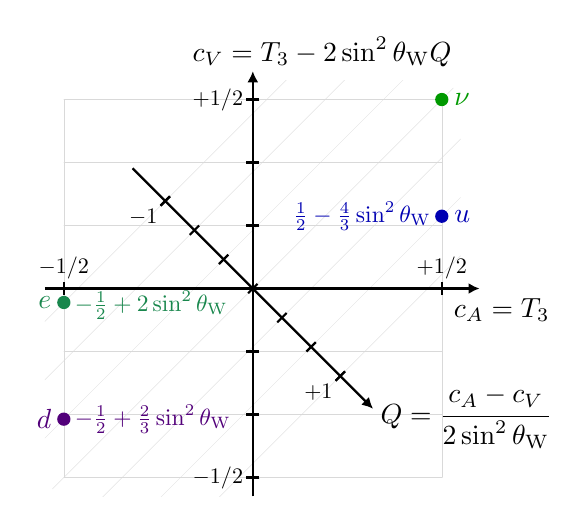
\begin{tikzpicture}[scale=2.4]
  \def\r{1.0pt} % point radius
  \def\thetaW{28.8} % weak mixing angle / Weinberg angle
  \def\sW{0.23153} % sin(theta_W)^2
  \def\sinthetaW{\sin^2\theta_\mathrm{W}}
  %\pgfmathsetmacro\sW{sin(\thetaW)^2} % sin(theta_W)
  \pgfmathsetmacro\qscale{4*\sW/(sqrt(2))} % unit Q charge in (I3,YW/2)
  
  % GUIDELINES
  \foreach \i in {2}{ % axial-vector cV coupling
    \draw[guide] (-\i/2,-1) -- (-\i/2,1);
    \draw[guide] ( \i/2,-1) -- ( \i/2,1);
  }
  \foreach \i in {1,...,3}{ % vector cA coupling
    \draw[guide] (-1,-\i/3) -- (1,-\i/3);
    \draw[guide] (-1, \i/3) -- (1, \i/3);
  }
  \begin{scope}
    \clip (-1.1,-1.1) rectangle (1.1,1.1);
    \foreach \i [evaluate={\q=\qscale*\i/3;}] in {-3,...,3}{ % EM charge Q
      \draw[guide,rotate=45] (-1.5,\q) -- (1.5,\q);
      \tick{135:\q}{45};
    }
  \end{scope}
  \foreach \i in {1,...,3}{ % ticks
    \tick{0,-\i/3}{0};
    \tick{0, \i/3}{0};
  }
  \begin{scope}[every node/.style={scale=0.8,inner sep=1}]
    \tick{-1,0}{-90} node[above] {$-1/2$};
    \tick{1,0}{-90} node[above] {$+1/2$};
    \tick{0,-1}{0} node[left] {$-1/2$};
    \tick{0,1}{0} node[left] {$+1/2$};
    \tick{-45:-\qscale}{45} node[below left] {$-1$};
    \tick{-45:\qscale}{45} node[below left] {$+1$};
  \end{scope}
  
  % AXES
  \draw[->,thick] (-1.1,0) -- (1.2,0) node[right=8,below] {$c_A = T_3$};
  \draw[->,thick] (0,-1.1) -- (0,1.15) node[right=25,above=-2] {$c_V = T_3 - 2\sinthetaW Q$};
  \draw[->,thick] (-45:-0.9) -- (-45:0.9) node[above=-2,right=-1] {$Q = \cfrac{c_A - c_V}{2\sinthetaW}$};
  
  % QUARKS
  \fill[mygreen]  ( 1, 1) circle(\r)
    node[right=1] {$\nu$};
  \fill[mygreen2] (-1,-1+4*\sW) circle(\r)
    node[left=1] {$e$}
    node[below=1,right=1,scale=0.85] {$-\frac{1}{2}+2\sinthetaW$};
  \fill[myblue]   ( 1, 1-8/3*\sW) circle(\r)
    node[right=1] {$u$}
    node[left=1,scale=0.85] {$\frac{1}{2}-\frac{4}{3}\sinthetaW$};
  \fill[mypurple] (-1,-1+4/3*\sW) circle(\r)
    node[left=1] {$d$}
    node[right=1,scale=0.85] {$-\frac{1}{2}+\frac{2}{3}\sinthetaW$};
  
\end{tikzpicture}


% LEPTOQUARK SU(2)_L x U(1)_Y QUANTUM NUMBERS
% Inspired by
%   "Physics of leptoquarks in precision experiments and at particle colliders"
%   I. Dorsner, S. Fajfer, A. Greljo, J. F. Kamenik, N. Kosnik
%   https://arxiv.org/abs/1603.04993
\begin{tikzpicture}[scale=3.5]
  
  % GUIDELINES
  \begin{scope}
    \clip
      (0,0.21) ellipse({1.12} and 1.3)
      (0,0.34) ellipse({1.12} and 1.4);
    \foreach \i in {1,2}{ % weak isospin T3
      \draw[guide] (-\i/2,-1.6) -- (-\i/2,1.6);
      \draw[guide] ( \i/2,-1.6) -- ( \i/2,1.6);
    }
    \foreach \i in {1,...,8}{ % weak hypercharge Y
      \draw[guide] (-1.2,-\i/6) -- (1.2,-\i/6);
      \draw[guide] (-1.2, \i/6) -- (1.2,\i/6);
    }
    \foreach \i in {-4,...,5}{ % charge Q
      \draw[guide,rotate=-45]
        (-1.3,\qscale*\i/3) -- (1.1,\qscale*\i/3);
    }
  \end{scope}
  \begin{scope}[
    every node/.style={scale=0.8,inner sep=1},
    qlab/.style={anchor=130,inner sep=0},
  ]
    \tick{-1,0}{90} node[below] {$-1$};
    \tick{-1/2,0}{90} node[below=-1] {$-\frac{1}{2}$};
    \tick{1/2,0}{90} node[below=-1] {$+\frac{1}{2}$};
    \tick{1,0}{90} node[below] {$+1$};
    \tick{0,-1}{0} node[left] {$-1$};
    \tick{0,-1/2}{0} node[left] {$-\frac{1}{2}$};
    \tick{0,1/2}{0} node[left] {$+\frac{1}{2}$};
    \tick{0,1}{0} node[left] {$+1$};
    \tick{0,3/2}{0} node[left] {$+\frac{3}{2}$};
    \tick{45:-4*\qscale/3}{135} node[qlab] {$-\frac{4}{3}$};
    \tick{45:-\qscale}{135} node[qlab] {$-1$};
    \tick{45:-2*\qscale/3}{135} node[qlab] {$-\frac{2}{3}$};
    \tick{45:-\qscale/3}{135} node[qlab] {$-\frac{1}{3}$};
    \tick{0,0}{135} node[below right=0] {$0$};
    \tick{45:\qscale/3}{135} node[qlab] {+$\frac{1}{3}$};
    \tick{45:2*\qscale/3}{135} node[qlab] {+$\frac{2}{3}$};
    \tick{45:\qscale}{135} node[qlab] {$+1$};
    \tick{45:4*\qscale/3}{135} node[qlab] {+$\frac{4}{3}$};
    \tick{45:5*\qscale/3}{135} node[qlab] {+$\frac{5}{3}$};
  \end{scope}
  
  % AXES
  \draw[->,thick] (-1.05,0) -- (1.1,0) node[right] {$T_3$};
  \draw[->,thick] (0,-1.05) -- (0,1.8) node[right=2,above=-2] {$\YW/2$};
  \draw[->,thick] (45:-1.1) -- (45:1.4) node[left=18,above right=-2] {$Q=T_3+\frac{1}{2}\YW$};
  
  % Scalar S3 (3,3,1/3)
  \drawtriplet[myred2,myred](1/3) node[right=2] {$S_3^i$};
  \fill[myred2]          (-1   ,1/3) circle(\r);
  \fill[myred!50!myred2] (-0.01,1/3) circle(\r);
  \fill[myred]           ( 1   ,1/3) circle(\r);
  
  % Scalar R2 (3,2,7/6)
  \drawdoublet[mypurple,myblue](7/6) node[right=2] {$R_2$};
  \fill[mypurple] (-1/2,7/6) circle(\r); %node[right=2,above=2] {$R_3$};
  \fill[myblue]   ( 1/2,7/6) circle(\r);
  
  % Scalar R2~ (3,2,1/6)
  \drawdoublet[mypurple,myblue](1/6) node[right=2] {$\tilde{R}_2$};
  \fill[mypurple] (-1/2,1/6) circle(\r); %node[right=2,above=2] {$\tilde{R}_3$};
  \fill[myblue]   ( 1/2,1/6) circle(\r);
  
  % Scalar S1~ (3,1,4/3)
  \fill[mygreen] (0,4/3) circle(\r) node[right=1] {$\tilde{S}_1$};
  
  % Scalar S1 (3,1,1/3)
  \fill[mygreen] (0.01,1/3) circle(\r) node[anchor=-135,inner sep=2] {$S_1$};
  
  % Scalar S1- (3,1,-2/3)
  \fill[mygreen] (0,-2/3) circle(\r) node[right=1] {$\overline{S}_1$};
  
  % Vector U3 (3,3,2/3)
  \drawtriplet[myred,myred2](2/3) node[below=0.5,right=2] {$U_{3\mu}^i$};
  \fill[myred]           (-1   ,2/3) circle(\r);
  \fill[myred!50!myred2] (-0.01,2/3) circle(\r);
  \fill[myred2]          ( 1   ,2/3) circle(\r);
  
  % Vector V2 (3,2,5/6)
  \drawdoublet[myblue,mypurple](5/6) node[below=0.5,right=2] {$V_{2\mu}$};
  \fill[myblue]   (-1/2,5/6) circle(\r);
  \fill[mypurple] ( 1/2,5/6) circle(\r);
  
  % Vector V2~ (3,2,-1/6)
  \drawdoublet[myblue,mypurple](-1/6) node[below=1,right=2] {$\tilde{V}_{2\mu}$};
  \fill[myblue]   (-1/2,-1/6) circle(\r);
  \fill[mypurple] ( 1/2,-1/6) circle(\r);
  
  % Vector U1~ (3,1,5/3)
  \fill[mygreen] (0,5/3) circle(\r) node[below=0.5,right=1] {$\tilde{U}_{1\mu}$};
  
  % Vector U1 (3,1,2/3)
  \fill[mygreen] (0.01,2/3) circle(\r) node[below=0.5,anchor=-145,inner sep=1.7] {$U_{1\mu}$};
  
  % Vector U1- (3,1,-1/3)
  \fill[mygreen] (0,-1/3) circle(\r) node[below=0.5,right=1] {$\overline{U}_{1\mu}$};
  
\end{tikzpicture}


\end{document}
